\subsection{Systemarchitektur}
Abbildung \ref{img:Systemarchitektur}: \glqq \nameref{img:Systemarchitektur}\grqq{} zeigt die Systemarchitektur des zu entwickelnden Systems. Es handelt sich um eine Server-Client-Architektur, bei der die Instanzen über die REST-API-Schnittstelle kommunizieren.
\begin{figure}[H]
	\centering
	\setlength{\fboxsep}{1pt}
	\setlength{\fboxrule}{1pt}
	\fbox{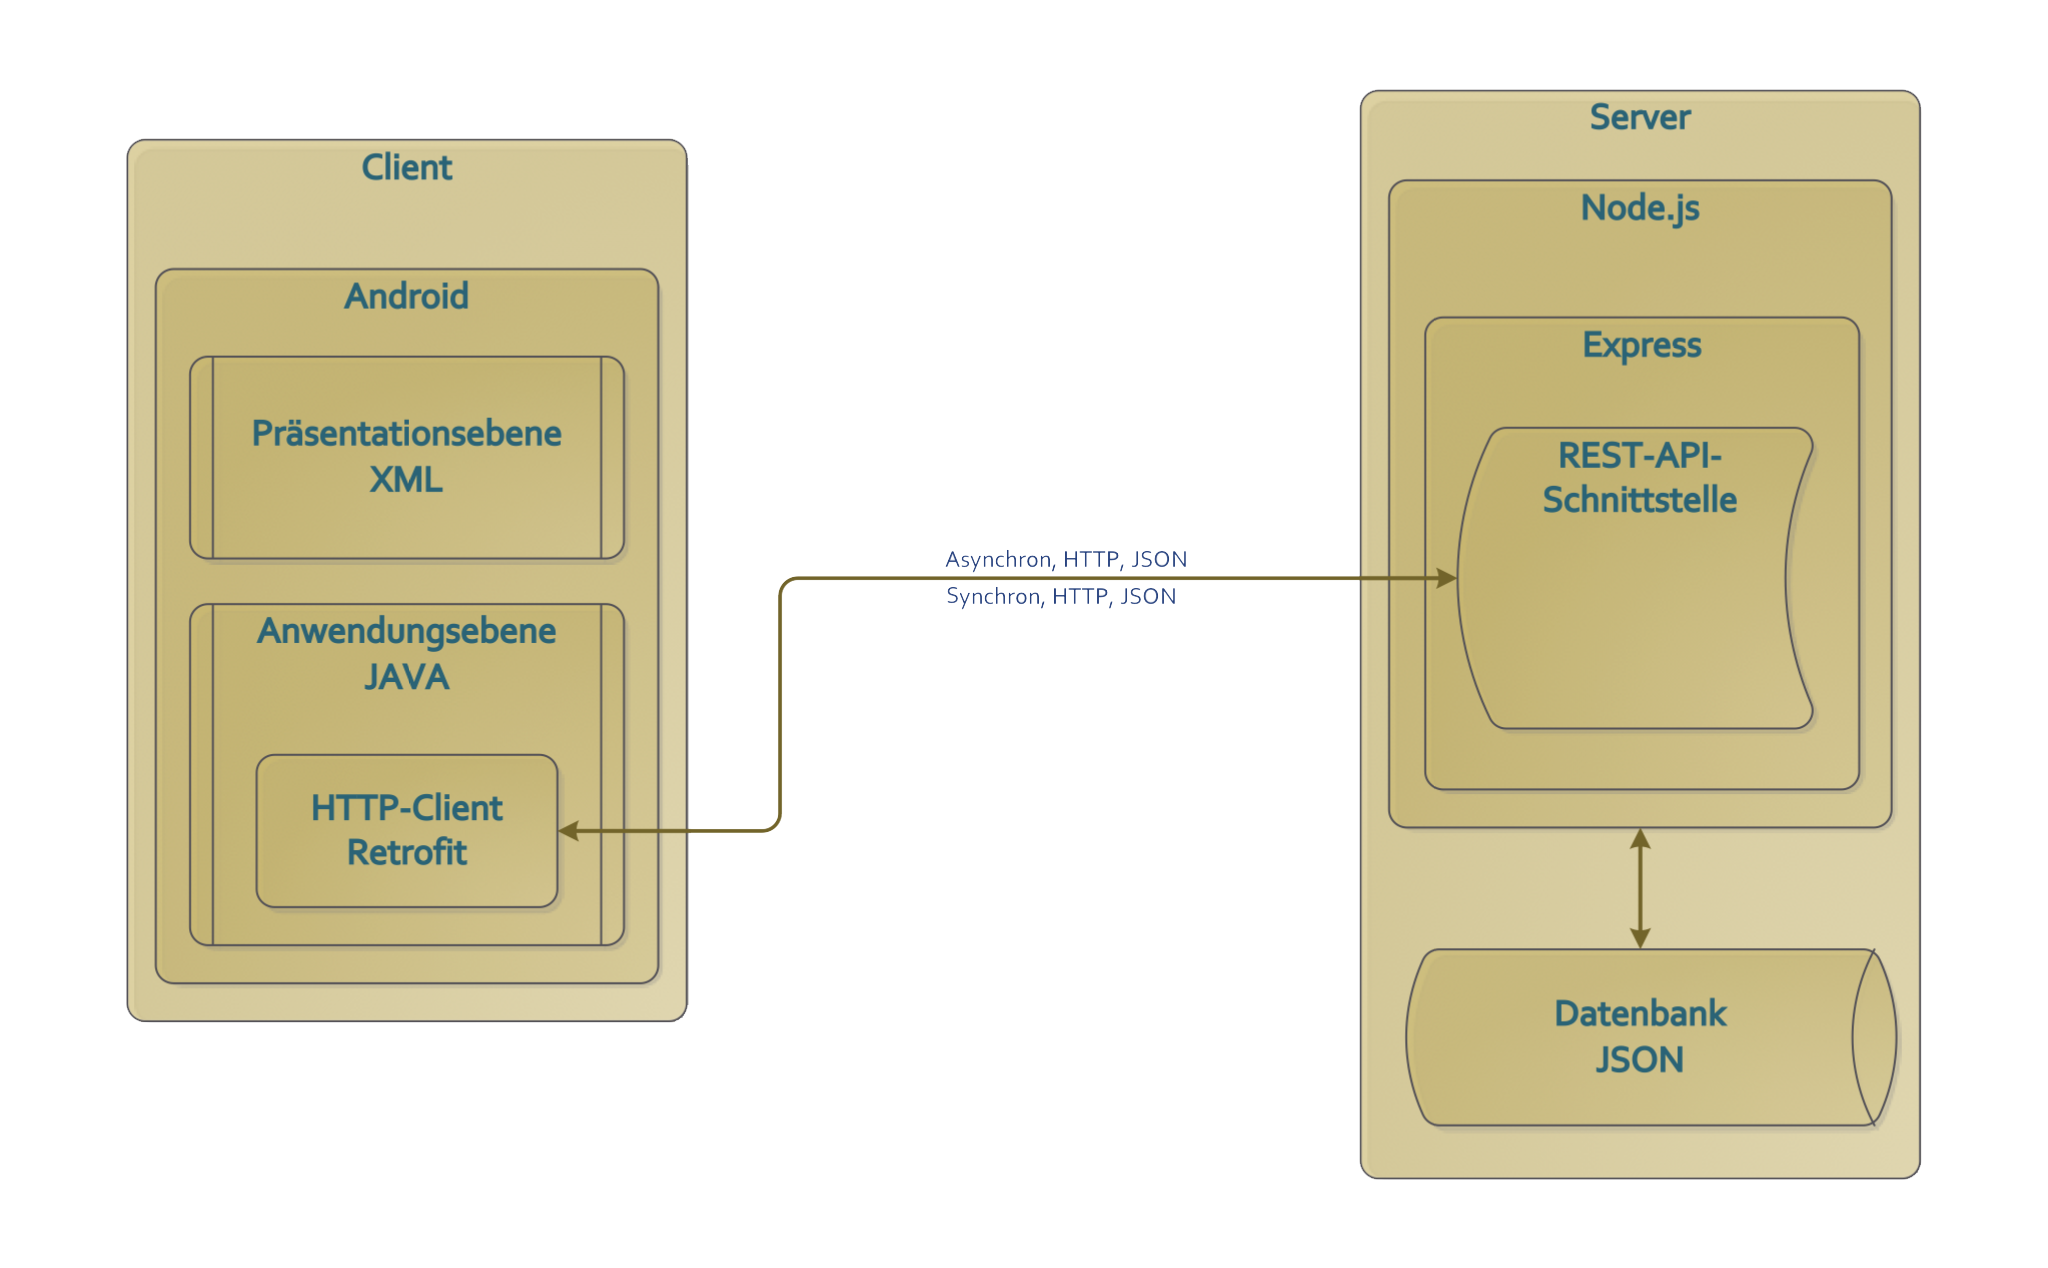
\includegraphics[width=1.0\textwidth]{images/systemarchitektur.png}}
	\captionsetup{justification=centering}
	\caption{Systemarchitektur}
	\label{img:Systemarchitektur}
\end{figure}
\subsubsection{Server-Client}
	In dem zukünftigen System für Android wird die Benutzeroberfläche von der Datenverwaltung getrennt. Dadurch kann das System in Zukunft plattformunabhängig sein. In weiteren Entwicklungsphasen könnte auch ein Client (Frontend) für das iOS-Betriebssystem implementiert werden, der ebenfalls mit dem Server (Backend) kommuniziert.\\
	Da eine direkte Kommunikation zwischen Systemkomponenten nicht erwünscht ist und kommunizierte Daten dauerhaft (persistent) und zentral gespeichert werden sollen, wurde eine Entscheidung gegen eine Peer-to-Peer-Architektur getroffen. Denn die Datenspeicherung für einzelne Komponenten wäre unsicher und würde ein Datenschutzrisiko darstellen.\\
	Die Client-Server-Architektur ist ebenfalls geeignet, da das System ein REST-spezifisches Design haben sollte. Zentrales Ressourcenmanagement ist eines der REST-Paradigmen, ermöglicht die Verwaltung vieler Benutzerdaten und gewährleistet einen bestimmten Sicherheitsstandard. Die Erweiterbarkeit, die diese Systemarchitektur ermöglicht, ist ein weiterer Grund, warum Client-Server als Architekturmodell ausgewählt wurde. 
\subsubsection{Server}
	Der Server ist das Zentrum des Systems und erledigt die Hauptarbeit. Kernaufgabe ist es, die vom Client empfangenen Daten in einer Datenbank zu speichern und danach mit Algorithmen zu prozessieren. Die Ergebnisse werden dem Client zur Verfügung gestellt. Der Server enthält eine REST-API-Schnittstelle über Framework Express.js, die für die Kommunikation mit dem Client verwendet wird. Die Entwicklung erfolgt in der Skriptsprache JavaScript in einer NodeJS-Umgebung.\\
	Aufgrund seiner unkomplizierten Struktur und Skalierbarkeit ist NodeJS ideal für das System. Darüber hinaus liegen bereits Erfahrungen in der Programmierung mit JavaScript und NodeJS aus der vorangegangenen Entwicklungsphase und der Implementierung eines Prototyps vor. Da das System REST-spezifisch sein sollte, ist die Verwendung von Framework Express.js geeignet.  
	\subsubsection{Client}
	Der Benutzer interagiert mit dem System über eine App auf seinem Android-Gerät und erhält eine Darstellung seiner verarbeiteten Daten. Bei der Implementierung der Benutzeroberfläche des Systems wurde eine Android-App anstelle einer Web-Anwendung ausgewählt. Dies scheint bei der Benutzer-System-Interaktion (user-system interaction) am sinnvollsten zu sein, da interaktive Arbeit am System ein einfacher und müheloser Vorgang ist, der in kurzer Zeit durchgeführt werden sollte, sodass eine Web-Applikation, die den Einsatz eines Browsers erfordert zu aufwendig wäre. Darüber hinaus müssen Webpages zunächst erstellt und für mobile Geräte optimiert werden und bei dem Umfang dieses Projektes wäre sogar ein Webserver erforderlich.\\
	Der Grund für die Wahl der Android-Plattform war auch die vorhandene Erfahrung mit Java. Retrofit eignet sich sehr gut als HTTP-Client für Android und Java. Er ist sehr flexibel im Design und ermöglicht das Senden und Empfangen von JSON- und XML-Dateien.\\
	Während die Anwendungsebene in Java programmiert wird, wird die Benutzeroberfläche des Clients durch XML dargestellt.
	\subsubsection{Datenbank}
	Die Datenbank ist mit dem Server verbunden und ermöglicht eine persistente Speicherung der Daten. Sie hostet Benutzerprofile und Benutzerereignisse und fungiert als Datenbanksystem für Lebensmittel- und Aktivitätsdaten.
	\subsubsection{Datenformat}
	Die Daten dieses Systems haben das JSON-Datenformat. JSON-Daten haben dieselbe Syntax wie JavaScript-Objekte, sodass die Verarbeitung der Daten in JavaScript einfach bleibt. JSON-Objekte können auch in Java gut verarbeitet werden, da passende Klassen implementiert werden können. Da der Server mit JavaScript und die Clients in Java programmiert sind, wurde entschieden, JSON zu verwenden. Zudem sind die verwendeten Daten nicht flexibel und immer fest strukturiert, weshalb auf die Verwendung von XML verzichtet wurde.
	\subsubsection{Protokolle}
	HTTP (HyperText Transfer Protocol) wird als Protokoll für die Datenübertragung verwendet, da der Server über eine REST-spezifische Architektur verfügt und JSON-Objekte über HTTP übertragen werden können.
	\subsubsection{Asynchrone und Synchrone Kommunikation}
	Die Kommunikation zwischen Server und Client kann sowohl synchron als auch asynchron erfolgen. Wenn der Benutzer Daten wie z. B. seine Blutzuckerwerte abrufen und anzeigen möchte, wird auf die nicht blockierende asynchrone Kommunikation zugegriffen, um sowohl bei erfolgreicher als auch bei fehlgeschlagener Anforderung ein Ergebnis zu erhalten. Beim Schreibvorgang, beispielsweise wenn der Benutzer ein neues Ereignis hinzufügt, erfolgt dies über eine synchrone Kommunikation.	
\subsection{Datenstrukturen}
	Die modellierten Datenstrukturen des Systems werden nachfolgend erläutert. Die dargestellten Datenstrukturen sind JSON-Objekte, für die auf dem Client entsprechende Klassen implementiert wurden.
	\subsubsection{Benutzerprofil}
	Ein Benutzerprofil enthält alle erforderlichen benutzerbezogenen Daten, die bei der Registrierung erstellt und später geändert werden können. Tagebucheinträge werden jedem zugeordneten Benutzer hinzugefügt. Für jeden dokumentierten Tag gibt es einen Eintrag mit einer ID, einem Datum und den Ereignissen. Ereignisse enthalten Informationen zu Uhrzeit, Blutzucker, Mahlzeit, BE/KE, Insulin-Einheiten und sportlicher Aktivität. Ein Datensatz für Mahlzeiten besteht aus einer Beschreibung und der Anzahl der Kalorien, Kohlenhydrate, Eiweiße und Fette. Sportliche Aktivitäten enthalten eine Beschreibung, die Dauer und die Anzahl der verbrannten Kalorien.
	\lstinputlisting{listings/benutzerprofil.json}
	\subsubsection{Beiträg und Kommentare}
	Ein Beitrag kann von einem Benutzer erstellt und von allen anderen Benutzern angezeigt werden. Um einem Benutzer einen Beitrag zuordnen zu können, erhält der Beitrag die Benutzer-ID und den Benutzernamen des Verfassers. Außerdem enthält jeder Beitrag seine zugehörigen Kommentare, die dieselbe Datenstruktur wie die Beiträge haben. Auf dem Client erbt die Comments-Klasse die Attribute der Post-Klasse. 
	\lstinputlisting{listings/beitrag.json}
	\subsubsection{Lebensmittel}
	Der Benutzer sollte in der Lage sein, seine Mahlzeiten zu dokumentieren. Dies erfordert eine Lebensmitteldatenbank, die verschiedene Lebensmittel enthält. Lebensmittel werden anhand ihrer ID, ihres Namens und ihrer Kategorie identifiziert und enthalten eine Menge und eine Einheit, anhand derer die Anzahl der Kalorien, Kohlenhydrate, Proteine und Fette bestimmt wird. Wenn der Benutzer die Menge der Mahlzeit angibt, werden die Nährstoffe basierend auf der Menge und der Einheit aus der Datenbank berechnet. 
	\lstinputlisting{listings/lebensmittel.json}
	\subsubsection{Sportart}
	Eine Sportartendatenbank soll es dem Benutzer auch ermöglichen, sportliche Aktivitäten zu dokumentieren. Um den Kalorienverbrauch einer Sportart zu berechnen, verwendet man das sogenannte metabolische Äquivalent (metabolic equivalent of task; MET). Ein MET entspricht einem Energieverbrauch von einer Kalorie pro kg Körpergewicht und Stunde. Eine Sportart besteht also aus ihrem Namen und der MET-Anzahl zur Berechnung des Kalorienverbrauchs.
	\lstinputlisting{listings/sportart.json}
		\newpage
\subsection{REST-Spezifikation}
	Die REST-Spezifikation des Servers befasst sich mit dessen Ressourcen und HTTP-Methoden, die im Folgenden erläutert werden.
	\subsubsection{Benutzer}
	\begin{itemize}
	\item Methode: POST\newline
	\noindent\hspace*{10mm} - Ressource: /users \newline
	\noindent\hspace*{10mm} - Semantik: Benutzerregistrierung \newline
	\noindent\hspace*{10mm} - Content-Type (req): application/json \newline
	\noindent\hspace*{10mm} - Content-Type (res): text/plain \newline
	\noindent\hspace*{10mm} - HTTP-Statuscode (erfolgreich): 201 Created \newline
	\noindent\hspace*{10mm} - HTTP-Statuscode (nicht erfolgreich): 406 Not Acceptable
	\item Methode: GET\newline
	\noindent\hspace*{10mm} - Ressource: /users \newline
	\noindent\hspace*{10mm} - Semantik: Alle Benutzer \newline
	\noindent\hspace*{10mm} - Content-Type (req): - \newline
	\noindent\hspace*{10mm} - Content-Type (res): application/json \newline
	\noindent\hspace*{10mm} - HTTP-Statuscode (erfolgreich): 200 OK \newline
	\noindent\hspace*{10mm} - HTTP-Statuscode (nicht erfolgreich): 404 Not Found
	\item Methode: PUT\newline
	\noindent\hspace*{10mm} - Ressource: /users/:userID \newline
	\noindent\hspace*{10mm} - Semantik: Benutzer bearbeiten \newline
	\noindent\hspace*{10mm} - Content-Type (req): application/json \newline
	\noindent\hspace*{10mm} - Content-Type (res): text/plain \newline
	\noindent\hspace*{10mm} - HTTP-Statuscode (erfolgreich): 200 OK\newline
	\noindent\hspace*{10mm} - HTTP-Statuscode (nicht erfolgreich): 404 Not Found, 406 Not Acceptable
	\item Methode: DELETE\newline
	\noindent\hspace*{10mm} - Ressource: /users/:userID \newline
	\noindent\hspace*{10mm} - Semantik: Benutzer löschen \newline
	\noindent\hspace*{10mm} - Content-Type (req): - \newline
	\noindent\hspace*{10mm} - Content-Type (res): text/plain \newline
	\noindent\hspace*{10mm} - HTTP-Statuscode (erfolgreich): 204 No Content\newline
	\noindent\hspace*{10mm} - HTTP-Statuscode (nicht erfolgreich): 404 Not Found
	\end{itemize}
	\subsubsection{Beitrag}
	\begin{itemize}
	\item Methode: POST\newline
	\noindent\hspace*{10mm} - Ressource: /posts \newline
	\noindent\hspace*{10mm} - Semantik: Beitrag verfassen \newline
	\noindent\hspace*{10mm} - Content-Type (req): application/json \newline
	\noindent\hspace*{10mm} - Content-Type (res): text/plain \newline
	\noindent\hspace*{10mm} - HTTP-Statuscode (erfolgreich): 201 Created \newline
	\noindent\hspace*{10mm} - HTTP-Statuscode (nicht erfolgreich): 406 Not Acceptable
	\item Methode: GET\newline
	\noindent\hspace*{10mm} - Ressource: /posts \newline
	\noindent\hspace*{10mm} - Semantik: Alle Beiträge \newline
	\noindent\hspace*{10mm} - Content-Type (req): - \newline
	\noindent\hspace*{10mm} - Content-Type (res): application/json \newline
	\noindent\hspace*{10mm} - HTTP-Statuscode (erfolgreich): 200 OK \newline
	\noindent\hspace*{10mm} - HTTP-Statuscode (nicht erfolgreich): 404 Not Found
	\item Methode: DELETE\newline
	\noindent\hspace*{10mm} - Ressource: /posts/:postID \newline
	\noindent\hspace*{10mm} - Semantik: Beitrag löschen \newline
	\noindent\hspace*{10mm} - Content-Type (req): - \newline
	\noindent\hspace*{10mm} - Content-Type (res): text/plain \newline
	\noindent\hspace*{10mm} - HTTP-Statuscode (erfolgreich): 204 No Content\newline
	\noindent\hspace*{10mm} - HTTP-Statuscode (nicht erfolgreich): 404 Not Found
	\end{itemize}
		\subsubsection{Lebensmittel}
	\begin{itemize}
	\item Methode: GET\newline
	\noindent\hspace*{10mm} - Ressource: /food \newline
	\noindent\hspace*{10mm} - Semantik: Alle Lebensmittel \newline
	\noindent\hspace*{10mm} - Content-Type (req): - \newline
	\noindent\hspace*{10mm} - Content-Type (res): application/json \newline
	\noindent\hspace*{10mm} - HTTP-Statuscode (erfolgreich): 200 OK \newline
	\noindent\hspace*{10mm} - HTTP-Statuscode (nicht erfolgreich): 404 Not Found
	\end{itemize}
\subsubsection{Sportart}
\begin{itemize}
	\item Methode: GET\newline
	\noindent\hspace*{10mm} - Ressource: /sport \newline
	\noindent\hspace*{10mm} - Semantik: Alle Sportarten \newline
	\noindent\hspace*{10mm} - Content-Type (req): - \newline
	\noindent\hspace*{10mm} - Content-Type (res): application/json \newline
	\noindent\hspace*{10mm} - HTTP-Statuscode (erfolgreich): 200 OK \newline
	\noindent\hspace*{10mm} - HTTP-Statuscode (nicht erfolgreich): 404 Not Found
	\end{itemize}
	Um Benutzer und Beiträge hinzufügen, anzeigen, bearbeiten oder löschen zu können, sind die oben genannten HTTP-Methoden erforderlich. Da Kommentare Teil eines Posts sind, können sie mit den HTTP-Methoden für \glqq Beitrag\grqq{} hinzugefügt, angezeigt und gelöscht werden. Gleiches gilt für Tagebucheinträge und Ereignisse. Diese sind benutzerspezifische Daten und können mit den HTTP-Methoden für \glqq Benutzer\grqq{} verwaltet werden.\newline
	Lebensmittel und Sportarten haben feste Datensätze, die nur gelesen, aber nicht gelöscht oder editiert werden können (GET-Methode).
	\subsection{Anwendungslogik}
	Um die einzelnen Funktionen jeder Systemkomponente zu verstehen, befasst sich der folgende Abschnitt mit der Anwendungslogik von Server und Client.
	\subsubsection{Client}
	Einige Java-Klassen mussten clientseitig implementiert werden. Dies sind zum einen die Klassen der Objekte, die auch serverseitig in der Datenbank gespeichert sind, und zum anderen die Helfer-Klassen wie die RestService-Klasse. Der Client kann anhand dieser Klassen und der JsonPlaceHolderApi-Schnittstelle mit dem Server kommunizieren. Beide Klassen sehen folgendermaßen aus:
	\lstinputlisting{listings/RestService.java}
	\lstinputlisting{listings/JsonPlaceHolderApi.java}
	Zusätzlich zu einigen Java-Klassen, die in der Dokumentation nicht beschrieben werden können, werden nachfolgend Funktionen und ihre Algorithmen erläutert. 
	\paragraph{BE/KE-Rechner}$~$\\
	Der BE/KE-Rechner wird verwendet, sobald der Benutzer ein Lebensmittel als Ereignis hinzufügt. Da die Anzahl der BE/KE nach der Berechnung vom Benutzer geändert werden kann, muss sie im Eingabe-Screen eines Ereignisses angezeigt werden. Hierfür wird ein TextWatcher verwendet, der diese aktualisiert, wenn die Mahlzeit und ihre Kohlenhydrate geändert werden. Der Programmcode sieht folgendermaßen aus: 
	\lstinputlisting{listings/beFactor_berechnung.java}
	\paragraph{Korrektureinheiten-Rechner}$~$\\
	Ein TextWatcher wurde auch für die Berechnung von Korrektureinheiten implementiert. Die Korrektureinheiten werden angepasst, wenn ein Blutzuckerwert eingegeben wird, der über dem Zielbereich des Benutzers liegt. Der Zielwert von 100 mg/dL wird vom überhöhten Blutzuckerwert abgezogen und die Differenz wird durch den Korrekturfaktor geteilt:
	\lstinputlisting{listings/korrektur_berechnung.java}
	\paragraph{Insulineinheiten-Rechner}$~$\\
	Zur Ermittlung der Insulineinheiten wird die Anzahl von BE/KE einer Mahlzeit mit dem BE/KE-Faktor des Benutzers multipliziert und die Korrektureinheiten werden dazu addiert:
	\lstinputlisting{listings/insulineinheiten_berechnung.java}
	\paragraph{Kalorienbedarf}$~$ \\
	Der Kalorienbedarf pro Tag eines Benutzers errechnet sich aus seinem Grund- und Leistungsumsatz. Die Grundumsatzrate wird basierend auf dem Körpergewicht, der Größe und dem Alter des Benutzers bestimmt. Der Leistungsumsatz wird durch die täglichen Aktivitäten definiert. Der Algorithmus dafür sieht wie folgt aus: 
	\lstinputlisting{listings/kalorienbedarf.java}$~$ \newline
	Mit der MPAndroidChart-Libary werden beispielsweise die Blutzuckerwerte in Form eines Grafen in einem Koordinatensystem dargestellt. Dazu müssen die Zeiten der Blutzuckermessungen zunächst in eine Dezimalschreibweise umgerechnet werden. Hierzu wurde eine eigene Methode implementiert.\newline
	Der Client berechnet auch den Kalorienverbrauch bei sportlichen Aktivitäten, die der Benutzer unter \glqq Ereignisse\grqq{} angibt. Er wird anhand des metabolischen Äquivalents (MET) der jeweiligen Sportart aus der Datenbank berechnet.\newline
	Der Client erstellt außerdem eine Highscore-Liste, in der die Benutzer mit den zehn höchsten Punktzahlen aufgeführt sind. Der Benutzer erhält Punkte, wenn er Ereignisse hinzufügt, Beiträge teilt oder kommentiert.  \newline
	Zum Abgleich von vom Benutzer eingegebenen Lebensmitteln mit der Lebensmitteldatenbank, wird ein TextWatcher verwendet. Bei einer Änderung oder Neuanlage wird nach dem neuen Lebensmittelnamen in der Datenbank gesucht. Wenn die Suche einen Treffer liefert, wird das bereits existierende Lebensmittel vorgeschlagen.\newline
	Zusätzlich zu den bereits vorgestellten Algorithmen verfügt der Client über viele andere Funktionen, von denen jedoch nicht alle aufgelistet werden können. 
	\subsubsection{Server}
	Neben der Kommunikation mit der Datenbank, dem Lesen und Schreiben in die Datenbank gehört die Datenverarbeitung (Data Processing) zu den Aufgaben eines App-Servers. Er berechnet Statistiken und überträgt Auswertungen basierend auf den Blutzuckerwerten des Benutzers. Zu diesem Zweck ruft der Server die Datensätze aus der Datenbank ab, berechnet den entsprechenden HbA1c-Wert, die Anzahl der Blutzuckerwerte im Zielbereich und den durchschnittlichen Blutzuckerwert und überträgt die aktualisierten Daten in die Datenbank.\newline
	Der Datenaustausch erfolgt auch zwischen Client und Server. Alle Clients in einem System zeigen den gleichen aktuellen Datenbestand an, da alle Daten in der Datenbank gespeichert sind und der Server sie dem Client auf Anfrage zur Verfügung stellt.
	 \lstinputlisting{listings/statics.js}$~$ \\
	 In Abbildung \ref{img:funktionsweise}: \glqq \nameref{img:funktionsweise}\grqq{} wird die Funktionsweise aller Instanzen im System veranschaulicht.
	 \begin{figure}[H]
	 \centering
	 \setlength{\fboxsep}{1pt}
	 \setlength{\fboxrule}{1pt}
	 \fbox{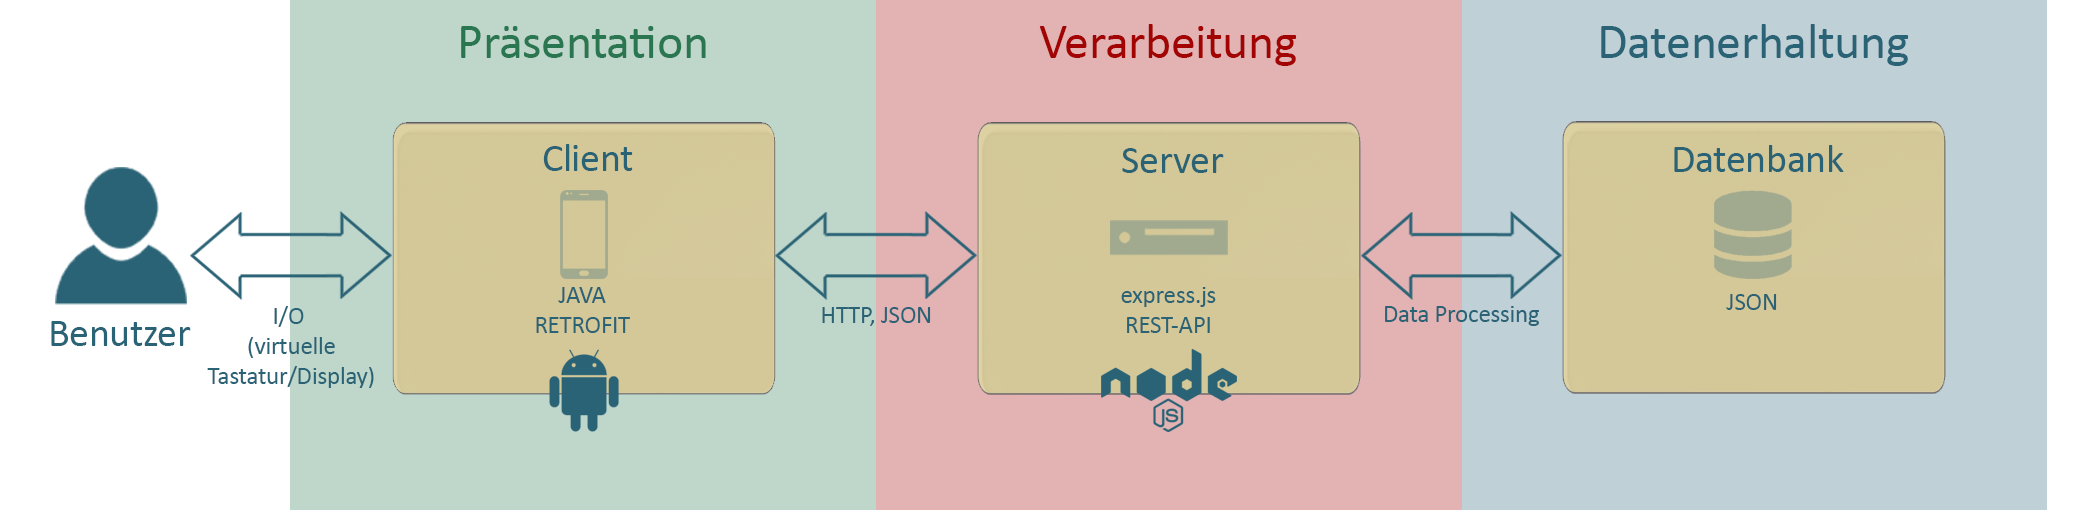
\includegraphics[width=1.0\textwidth]{images/funktionsweise.png}}
	 \captionsetup{justification=centering}
	 \caption{Funktionsweise}
	 \label{img:funktionsweise}
	 \end{figure}
	 \subsection{Installationsdokumentation}
	 Um das System erfolgreich zu installieren, muss das GitHub-Repository zuerst geklont werden. Das Repository kann mit dem folgenden Befehl in die Shell geklont werden:\\	 
	 \textit{\$ git clone https://github.com/sami1905/BAWS1920Hassini}\\
	 Nun folgt die Beschreibung, mit der Server und Client installiert werden können.
	 \subsubsection{Server}
	 1. Starte die Shell und öffne den Pfad:\\
	 \textit{/Implementation/DiaLog/Server}\\
	 2. Starte den Server mit dem Befehl:\\
	 \textit{\$ node app.js}\\
	 3. Sobald die Meldung \textit{\glqq Server läuft auf Port 3000.\grqq{}} in der Shell erscheint, ist der Server erfolgreich installiert und gestartet.
	  \subsubsection{Client}
	  1. Android Studio starten und den Odner \textit{Client} aus dem Repository öffnen.\\
	  2. Ein Virtual Device einrichten.\\
	  3. Emulator starten.\\
	  4. Um das System nutzen zu können, werden folgende Zugangsdaten verwendet:\newline
	  \textbf{E-Mail-Adresse: }\textit{\glqq m.mustermann@th-koeln.de\grqq{}} \newline
	  \textbf{Passwort: }\textit{\glqq 12345678\grqq{}}
	
